%
% Florent JACQUET - Romain THIBAUD - Antonin WALTZ
%
% Rapport de IN55 (P16)
%   Animation d'un personnage 3D avec OpenGL
%
%

\documentclass[a4paper]{report}
%packages
\usepackage[utf8]{inputenc}
\usepackage[francais]{babel}
\usepackage{graphicx}\graphicspath{{img/}}
\usepackage{float}
\usepackage[T1]{fontenc}
\usepackage{color}
\usepackage{fancyhdr}
\usepackage{listings}
\usepackage[colorlinks=true,allcolors=black]{hyperref}
\usepackage[font=small,labelfont=bf,margin=\parindent,tableposition=top]{caption}
\setcounter{tocdepth}{2}

\begin{document}
\begin{titlepage}
    
\includegraphics[width=0.4\textwidth]{logo_utbm.png}
    \begin{center}
        \textsc{\LARGE Université de Technologie de Belfort Montbéliard}\\[1cm]
        \textsc{\Large IN55}\\
        \rule{\linewidth}{0.5mm}
        { \huge \bfseries Animation d'un personnage 3D avec OpenGL\\[0.4cm] }
        \rule{\linewidth}{0.5mm}
        \vskip1cm
        % Author and supervisor
        Florent \textsc{Jacquet}\\
	Romain \textsc{Thibaud}\\
        Antonin \textsc{Waltz}\\
        Superviseur: Fabrice \textsc{Lauri}\\
        \vskip1cm
        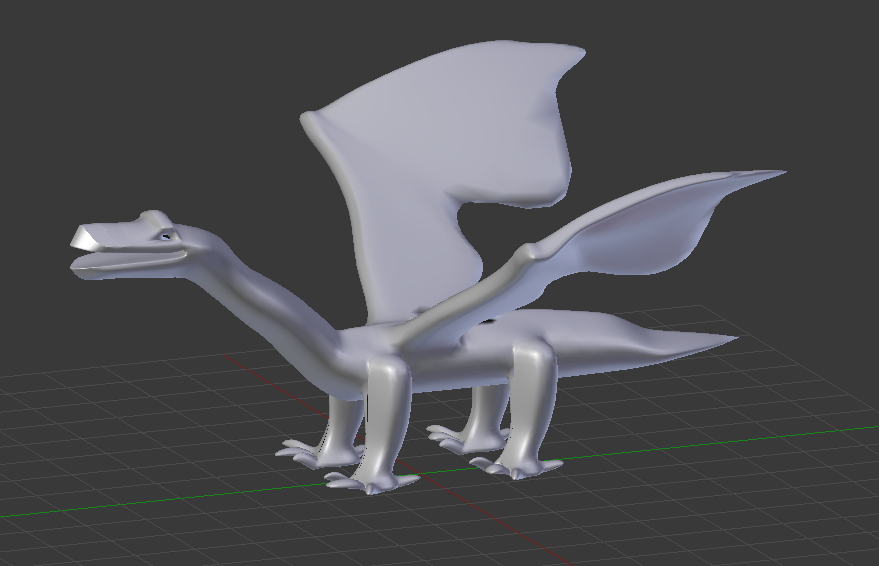
\includegraphics[width=0.6\textwidth]{dragon_front_page.png}
        \vfill
        {\large Printemps 2016}
    \end{center}
\end{titlepage}

\newpage
\tableofcontents
\listoffigures
\newpage
%%%%%%%%%%%%%%%%%%%%%%%%%%%%%%%%%%%%%%%%%%%%%%%%%%%%%%%%%%%%%%%%%%%%%%%%%%%%%%%%%%%%%%%%%%%%%%%%%%%%%%%
\chapter{Présentation du projet}
\par

Durant ce semestre en IN55, nous avons choisi le projet \textit{Animation d'un personnage 3D} parmi tout ceux proposés. Le personnage que nous avons choisi de modéliser et d'animer est un dragon. Les raisons de ce choix sont multiples. 

Tout d'abord, étant tous plus ou moins proche des communautés fan d'heroic-fantasy, le dragon est pour nous une figure emblématique de notre imaginaire. Ce projet nous laisser donc l'opportunité de donner vie à cette créature mythique. 

Dans un second temps, c'est l'architecture du squelette qui nous a donné envie. Basiquement, un dragon c'est : une tête, un cou, un buste, des ailes, des pattes et une queue. Cette structure nous a paru suffisament complexe pour que l'on puisse faire des animations intéressantes, mais reste relativement simple n'ayant pas forcément trop d'éléments du squelette qui se suivent. Ainsi, nous avons voulut faire voler, marcher ou s'asseoir notre dragon.

Nous developperons dans ce rapport la structure de notre objet 3D. Nous parlerons aussi des technologies employées pour faire le rendu 3D et de l'architecture de notre programme. Enfin, nous ouvrirons des pistes d'évolution pour ce projet. 


\newpage
%%%%%%%%%%%%%%%%%%%%%%%%%%%%%%%%%%%%%%%%%%%%%%%%%%%%%%%%%%%%%%%%%%%%%%%%%%%%%%%%%%%%%%%%%%%%%%%%%%%%%%%
\chapter{Modélisation et armature}
\par
Nous avons effectué la modélisation du dragon sous Blender. Nous avons choisis ce logiciel pour plusieurs raisons. D'abord son accessibilité, il est plus intuitif qu'une grande partie de ses concurrents (Maya ou 3DsMax) et permet donc d'avoir des résultats convaincants plus rapidement. Ensuite il a l'avantage d'être libre et gratuit, nous n'avons donc pas eu besoin de pirater un logiciel ou d'utiliser des licenses étudiantes contraignantes, et nous avons notamment le droit de montrer notre projet. Ceci est relativemment important pour nous, étant donné que nous sommes en dernière année, il est primordial de pouvoir partager nos réalisations dans le cadre de recherche de stage ou d'emploi. Cependant, la suite d'Autodesk (Maya ou 3DsMax) étant majoritairement utilisée dans l'industrie et le divertissement, nous ne sommes pas formé sur ces logiciels en choisissant Blender.

Son armature se découpe en plusieurs parties indépendantes les unes des autres. Il y a :
\begin{itemize}
\item La machoire haute (1 os)
\item La machoire (1 os)
\item Le cou (6 os)
\item Le corps allant de la base du coup jusqu'à la queue (8 os)
\item Les ailes, indépendantes (13 os par aile)
\item Les pattes, indépendantes également (6 os par patte)
\end{itemize}

Chaque partie est composée de plusieurs os reliés entre eux. Chaque os dispose d'une position et d'une orientation qui dépends de celle de son parent. Sous Blender nous avons utilisé des Inverse Kinematics Bones pour les pattes et les ailes en particulier. En procédant ainsi, un mouvement fluide est obtenu.

\begin{figure}[H]
    \begin{center}
        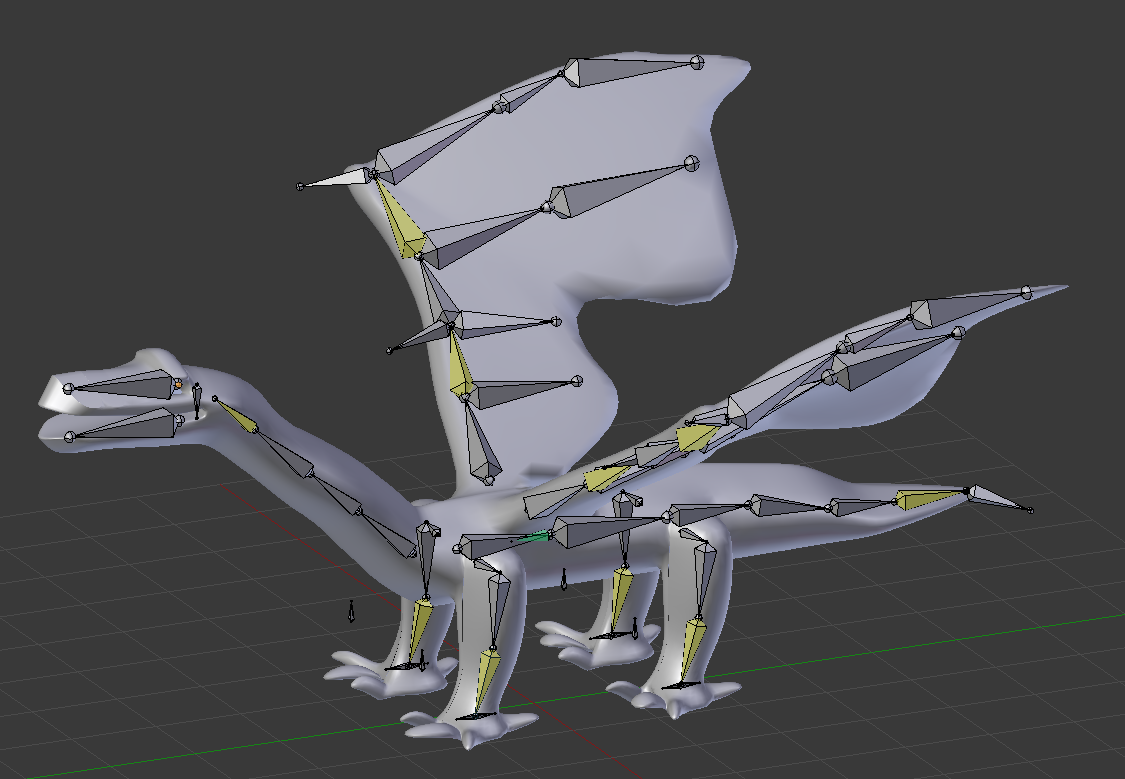
\includegraphics[width=0.85\textwidth]{armature.png}
        \caption{Armature}
    \end{center}
\end{figure}
\newpage
%%%%%%%%%%%%%%%%%%%%%%%%%%%%%%%%%%%%%%%%%%%%%%%%%%%%%%%%%%%%%%%%%%%%%%%%%%%%%%%%%%%%%%%%%%%%%%%%%%%%%%%

\chapter{Architecture du projet}
\section{Choix technologiques}
De part le sujet du projet, nous devions effectuer le rendu 3D à l'aide d'un programme alliant C++ et OpenGL. Il était conseillé de le faire avec Qt, un framework C++ qui offre diverses bibliothèques et widgets pratique pour mettre en oeuvre des applications C++. Cependant, après de nombreux problèmes dus aux différentes plateformes de développement que nous possédions, nous avons essayer avec la bibliothèque Open GL Utils (qui est très liée à Open GL). Cela nous a permis de faire ce que nous souhaitions et donc nous nous sommes passés de QT.
\section{La librairie Asset Import} 
\par
Asset Import est une librairie libre sous licence BSD permettant d'importer dans une structure de données un très grand nombre de fichiers 3D. Elle offre plusieurs avantage, comme le fait d'avoir une API pour du C++ ou du C, ou encore de pouvoir exporter des modèles 3D. Elle est d'ailleurs la base d'une visionneuse 3D disponible sur windows : open3mod (qui est open source). Lors de la modélisation sous Blender, nous n'avions pas à nous préoccupé particulièrement de comment gérer les formes compliquées ou les normales de toutes les faces. Or, lors du parsage du fichier exporté, nous devons nous en préoccuper.
\par
L'utilisation de Asset Import a permis de s'affranchir des opérations bas-niveau de parsage de fichier, ainsi que de la vérification 
syntaxique du fichier 3D, tout en permettant de faire des tests avec un très grand nombre possible de 
fichiers comme le Collada, le FBX, le format 3DS, l'OBJ ou même si on le souhaite des format plus exotiques comme le BVH (un format de motion capture) ou le .3d (un format utilisé par le moteur de jeu Unreal).
\par
Ces fichiers supportant différentes fonctionnalités, il n'est toutefois pas toujours possible de visualiser les animations.

\section{Nos structures de données}
\par
Si la librairie assimp permet de charger le fichier en mémoire dans une structure de données, elle ne permet 
cependant pas de faire de l'animation squelettale directement. Il faut donc soit faire une fonction capable 
de parcourir la structure rapidement, afin d'extraire les bonnes informations pour ensuite les afficher, mais
cette solution est très couteuse en terme de temps de calcul, puisqu'en plus de faire les calculs
d'interpolation, il faut aussi gérer le parcours de structure complexe.
\par
Nous avons donc décider de faire nos propres structures de données, plus simples, et donc moins exhaustives,
mais suffisantes pour les besoins du projet, tout en nous donnant une maitrise totale sur les options de rendus et d'animations.
\par
Des fonctions de chargement sont donc appellées au lancement, récupérant les informations requises grâce à 
assimp, pour pouvoir ensuite y accéder rapidement et simplement.

\subsection{Les structures principales}
\par
On trouve généralement dans un fichier une scène contenant plusieurs objets.

\begin{itemize}
\item $SceneHandler$ : C'est la classe centrale qui contient toutes les informations.
\item $Mesh$ : Un $Mesh$ est une structure qui contient principalement une liste de $vertex$, de $bones$ et de $faces$. L'orientation de ces faces est définie par leur normale, comprise également dans le $mesh$.
\item $Vertice$ : Un $Vertices$ contient un $vertex$ avec deux tableaux de taille 4. Le premier détaille les $Bones$ qui influent sur lui. Le second mesure le poids d'influence.
\item $Bones$ : Un $Bones$ contient un $bone$ et la liste des $vertex$ sur lesquels il influe.
\item $Face$ : Une $Face$ contient une liste d'indice qui forment une face.
\item $Animation$ : Une $Animation$ contient une liste de $BoneAnim$. Il y a autant de liste que de $Bone$.
\item $BoneAnim$ : Une $BoneAnim$ contient 3 listes qui correspondent aux clés pour la translation, la rotation et la mise à l'échelle.
\item $BoneState$ : Une $BoneState$ contient l'état d'un $Bone$
\item $VectInterpolation$ et $RotInterpolation$ : Ces deux classes s'occupent de l'interpolation des matrices de transformation entre deux $KeyFrame$ (moment clé d'une animation)
\end{itemize}

\subsection{Caméra libre}
\par
La caméra libre dispose de 5 degrès de liberté. Tout d'abord les 3 translations de l'espace sont possibles. Ainsi les flèches du haut et bas nous permette de se déplacer sur l'axe $y$ (axe vertical) pendant que celle de droite et gauche nous translate selon $x$ (axe horizontale) enfin la molette de la souris contrôle le mouvement suivant $z$ (la profondeur). Ensuite 2 rotations sont disponibles. Un clique gauche souris maintenue suivi d'un déplacement permet de tourner autour de l'axe vertical tandis que la même manipulation avec un clique droit permet une rotation autour de l'axe horizontal. La rotation autour de l'axe de profondeur n'ayant que peu d'intérêt, elle n'a pas été implémenté. 

Le fonctionnement est relativement simple, il y a un $eventListenner$ qui écoute les commandes claviers, un autre pour celle de la souris et un dernier pour les mouvements de la souris. Si un de ces trois éléments reçoit un stimuli, il met à jour la position et ou l'orientation de la caméra, et le rendu de cette dernière sera effectué au prochain rafraîchissement de l'affichage. 

\newpage
%%%%%%%%%%%%%%%%%%%%%%%%%%%%%%%%%%%%%%%%%%%%%%%%%%%%%%%%%%%%%%%%%%%%%%%%%%%%%%%%%%%%%%%%%%%%%%%%%%%%%%
\chapter{Diagramme de classe}
\section{Mesh Structure}
\begin{figure}[H]
    \begin{center}
        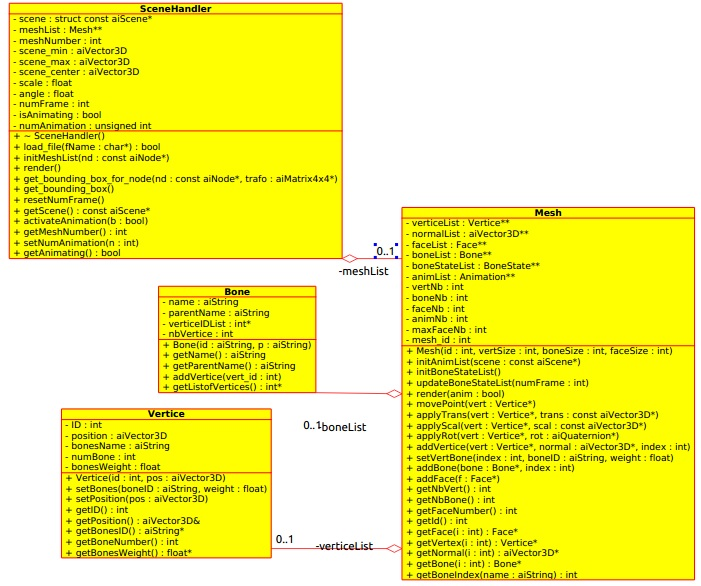
\includegraphics[width=1\textwidth]{MeshStructure.jpg}
        \caption{Diagramme de classe pour la structure d'un Mesh}
    \end{center}
\end{figure}
    La structure de Mesh est ce qui nous permet d'effectuer le rendu de notre objet. Elle est composée d'une liste de bone et une de vertice. On peut ainsi savoir qui est lié à qui. De plus, dans chaque verice on stocke aussi l'importance des bones sur lui dans le tableau de Weights. Le nombre de bones est volontairement limité à 4 pour alléger un peu les calculs, et d'après l'avis de plusieurs utilisateur de la biliothèque ce nombre est suffisant. 

    Il y a aussi une liste de face qui permet de savoir quels vertices forme quel polygone. On stocke avec les normal à chaque face ce qui est très utile pour les rendus d'illuminations par exemple.

    La fonction qui procède au rendu est la fonction render. Dans le SceneHandler on appel cette fonction pour chaque Mesh qui va parcourir la liste des faces afin d'en effectuer le rendu. C'est d'ailleurs ici, que l'on effectue les transformations apportées aux vertices lors de l'animation afin d'en fair ele rendu.

    Toute nos listes sont initialisée grace à la méthode initMeshList de SceneHandler et ce avant le premier rendu ce qui nous permet d'effectuer certain calcul en amont. D'où l'intéret de se servir de nos propres structures.

    \section{Animation Structure}

\par


\newpage
%%%%%%%%%%%%%%%%%%%%%%%%%%%%%%%%%%%%%%%%%%%%%%%%%%%%%%%%%%%%%%%%%%%%%%%%%%%%%%%%%%%%%%%%%%%%%%%%%%%%%%
\chapter{Bilan}
\section{Guide d'utilisation}
Voici les touches à utiliser pour manipuler le programme :
\begin{description}
	\item[1,2,3 :] Sélectionne et lance une animation.
	\item[$\leftarrow,\uparrow,\downarrow,\rightarrow$ :] Translate la caméra sur les axes $X$ et $Y$
	\item[Souris :] Maintenir un clic et déplacer la souris déplacera la caméra libre sur l'axe en question.
	\item[Molette souris :] Avancer ou reculer la molette déplacera la caméra de façon à zoomer/dézoomer.
\end{description}
\section{Difficultés rencontrées}
\par
Durant ce projet, nous avons été confronté à plusieurs difficultés :
\begin{itemize}
\item La prise en main des Inverse Kinematics pour avoir un rendu acceptable des animations dans Blender a été laborieuse.
\item Il nous a fallut un temps d'adaptation pour prendre en main et comprendre comment utiliser la librairie Assimp.
\item Comprendre comment parcourir de grandes quantités de données à travers des structures complexes pleines de références croisées a également été un frein à l'avancé du projet.
\item De manière générale, la gestion de la mémoire en C++.
\end{itemize}
\section{Améliorations possibles}
\par
En l'état il existe plusieurs types d'améliorations qui pourraient être apportées au projet. Tout d'abord, on pourrait texturer notre modèle. Actuellement on reconnait la forme d'un dragon mais pas l'aspect. En rajoutant une texture et des $normal map$ et autres $bump map$, on pourrait donner un aspect reptilien à la surface du dragon, affiner certains aspects et rajouter des formes sans pour autant qu'il y ait plus de polygones. Cela impliquerait de mettre en oeuvre des Shaders pour effectuer les calculs d'illuminations par exemple. 

Les Shaders pourraient aussi nous aider à affiner l'animation en allégeant la charge de calcul du CPU en se servant du GPU pour appliquer les transformations. En effet, le parcours de strcuture suivit du calcul des tranformations allourdit la charge de calcul, et en déléguant au GPU on pourrait alors charger des scènes plus lourdes et que cela reste fluide. 

La caméra libre pourrait aussi être améliorée, son utilisation est actuellement un peu rude, surtout au niveau des rotations. Il s'agirait de modifier les valeurs de modification de la position et de la rotation. Par exemple, pour la rotation, on base le changement sur l'amplitude du mouvement de la souris, celui-ci mériterait d'être traiter pour que se soit plus agréable et on pourrait rajouter une zone de non-action autour du curseur, afin qu'un petit tremblement ne bouge pas la caméra.

\section{Conclusion}
\par
Pour conclure, ce projet a été l'occasion de découvrir la programmation graphique avec OpenGL et l'utilisation de librairies gravitant autour de la 3D. Travailler sur un dragon et le voir s'animer au fil du temps a rendu le projet particulièrement ludique.
Nous avons pu appréhender le processus de modélisation et d'animation d'un personnage pour arriver à la représentation du rendu dans une scène. Nous avons pu constater comment appliquer les concepts vus en cours. Explorer les différentes possibilités offertes par des librairies libres nous a aussi forcer à aller chercher ce qu'il est possible de faire et comment le réaliser avec ces outils mis à notre disposition.


\newpage
%%%%%%%%%%%%%%%%%%%%%%%%%%%%%%%%%%%%%%%%%%%%%%%%%%%%%%%%%%%%%%%%%%%%%%%%%%%%%%%%%%%%%%%%%%%%%%%%%%%%%%
\chapter{Annexes}

\end{document}


